\documentclass[10pt]{article}
\usepackage[spanish]{babel}
\usepackage[utf8]{inputenc}
\usepackage[T1]{fontenc}
\usepackage{FiraSans}
\usepackage{amsmath}
\usepackage{graphicx}
\usepackage{float}
\usepackage{subfig}
\usepackage{array}
\usepackage{geometry}
\usepackage[shortlabels]{enumitem}
\renewcommand{\familydefault}{\sfdefault}
\renewcommand{\arraystretch}{1.1}

\geometry{margin=1in}
\begin{document}

\begin{titlepage}
\newcommand{\HRule}{\rule{\linewidth}{0.5mm}} 
\center


\includegraphics[scale=0.4]{images/logo-usm.png}\\
\vspace{0.6cm}
\textsc{\large INF480}\\[0.5cm] % Minor heading such as course title
\textsc{\Large Redes Complejas}\\[0.5cm] % Major heading such as course name

\HRule \\[0.4cm]
{ \huge \bfseries Tarea 3}\\[0.4cm] % Title of your document
\HRule \\[1.5cm]
 
\begin{minipage}{0.8\textwidth}
\begin{center} \large
Florencia Ramírez, ROL: 202073522-0\\
Sofía Riquelme, ROL: 202073615-4
\end{center}

\end{minipage}\\[2cm]

\vfill 

\end{titlepage}
\begin{itemize}
    \item \textbf{Pregunta 1}\\
        Se generaron dos redes, una Erdös-Renyi y otra Barabási-Albert, con grado promedio 2. Luego de completar el experimento en 1000 iteraciones, se obtuvo lo siguiente:
        \begin{figure}[H]
            \centering
            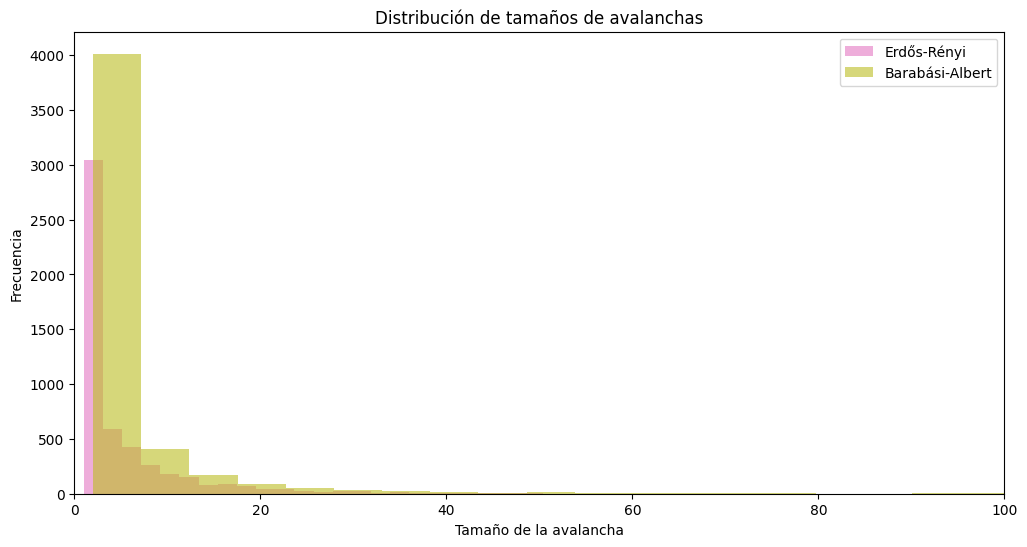
\includegraphics[scale=0.55]{images/avalancha.png}
            \caption{Distribución de avalanchas}
            \label{fig:grafico_avalancha}
        \end{figure}
        Es posible notar que en ambos caso la distribución muestra que la mayoría de las avalanchas son pequeñas, y como cae rápidamente su frecuencia a medida que aumenta el tamaño de la avalancha. Se puede ver que para ambos casos, se sigue una ley de potencia: $$P(x) \sim x^{-\alpha}$$Posterior a esto se hizo un código para estimar el parámetro $\alpha$ y se obtuvo que el que mejor se ajustaba es $\alpha = 4.07$ para la red Erdös-Renyi y $\alpha = 2.66$ para la red Barabási-Albert, como se muestra en la figura a continuación:
        \begin{figure}[H]
            \centering
            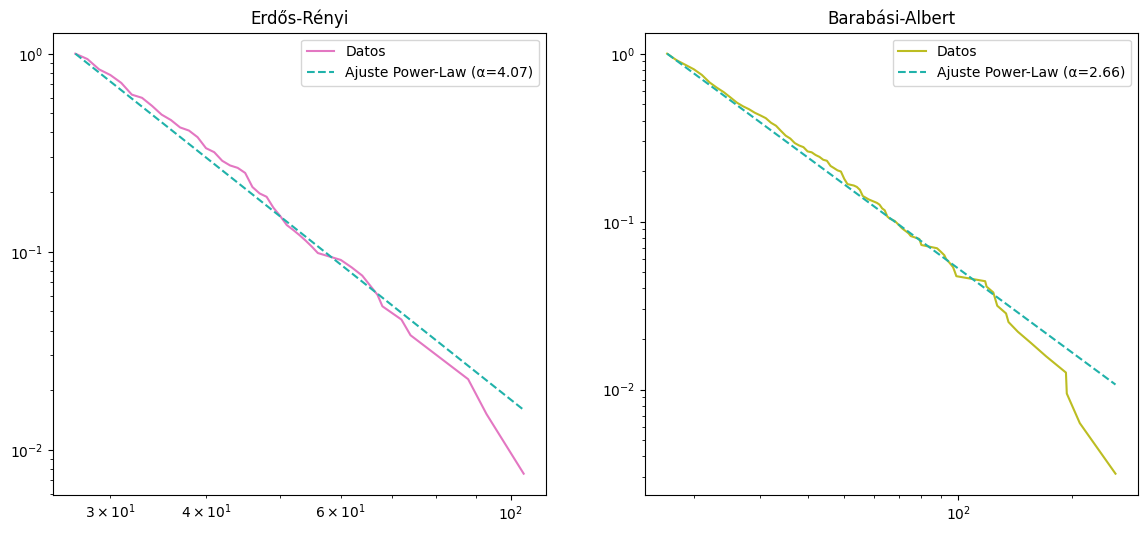
\includegraphics[scale=0.55]{images/grafico_ajuste.png}
            \caption{Distribución de avalanchas}
            \label{fig:grafico_distribucion}
        \end{figure}
        \newpage
    \item \textbf{Pregunta 3}
        \begin{enumerate}[(a)]
            \item La evolución del grado promedio, la transitividad y la modularidad se puede ver a continuación:
            \begin{figure}[H]
                \centering
                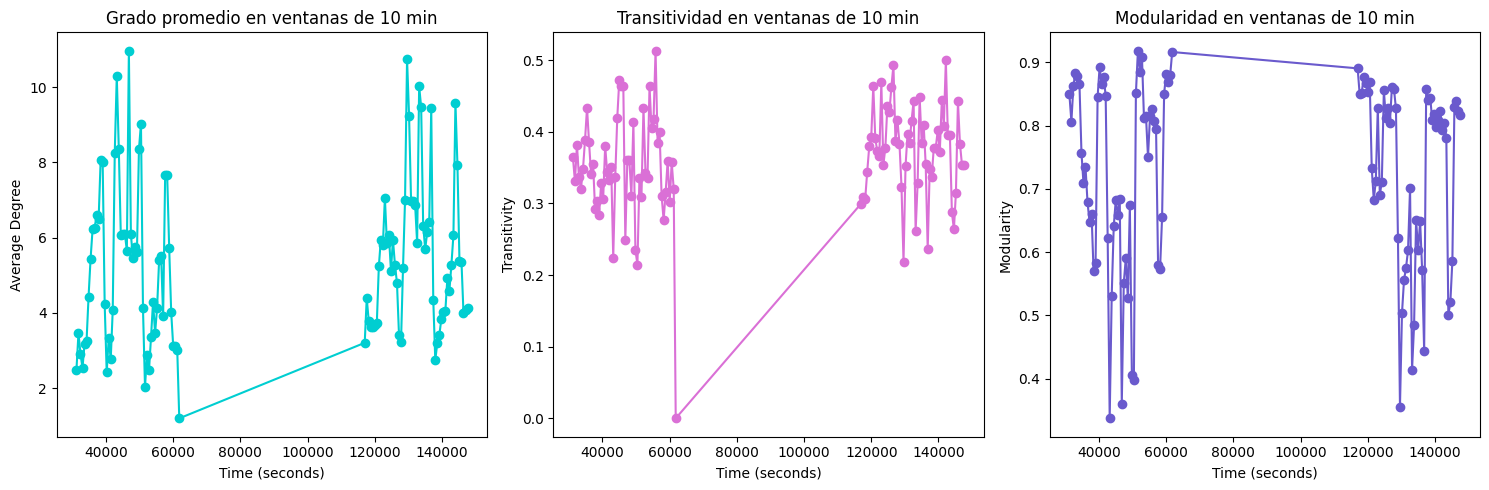
\includegraphics[scale=0.4]{images/10min.png}
                \caption{Evolución en ventanas de 10 minutos}
                \label{fig:grafico_10min}
            \end{figure}

            \begin{figure}[H]
                \centering
                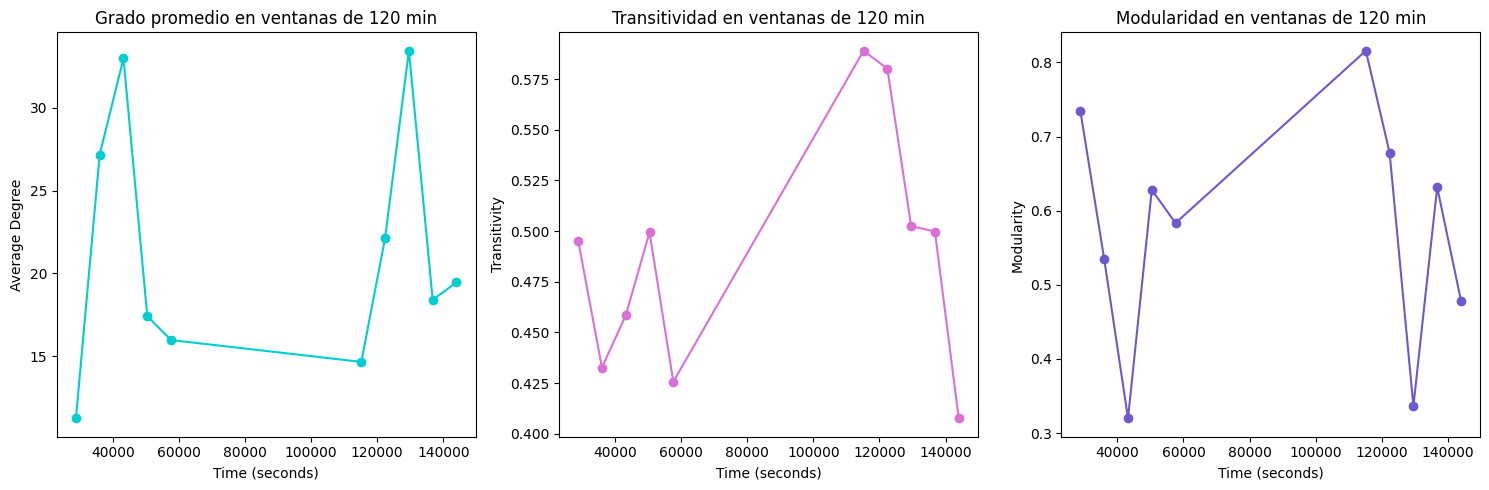
\includegraphics[scale=0.4]{images/120min.png}
                \caption{Evolución en ventanas de 120 minutos}
                \label{fig:grafico_120min}
            \end{figure}

            Respecto al grado promedio, fluctúa considerablemente en ventanas de tiempo cortas. Cuando es más alto, puede representar un momento específico del día, como un recreo. En el gráfico de ventanas de 120 minutos, se ven más suavizadas las fluctuaciones rápidas y se ve con más claridad los momentos más altos. 

            La transitividad fluctúa bastante, pero al igual que el grado promedio se observan momentos específicos donde es más alta. Sin embargo, tiende a ser más alta en intervalos largos, lo que sugiere que a largo plazo es más probable que se formen comunidades densas y cerradas.

            En el caso de la modularidad, es la que más fluctúa de las tres métricas. Esto sugiere que las comunidades dentro de esta red varían rápidamente, lo cual se evidencia en ambos gráficos.
            \newpage
            \item El tamaño del conjunto de influencia se puede ver a continuación:
            \begin{figure}[H]
                \centering
                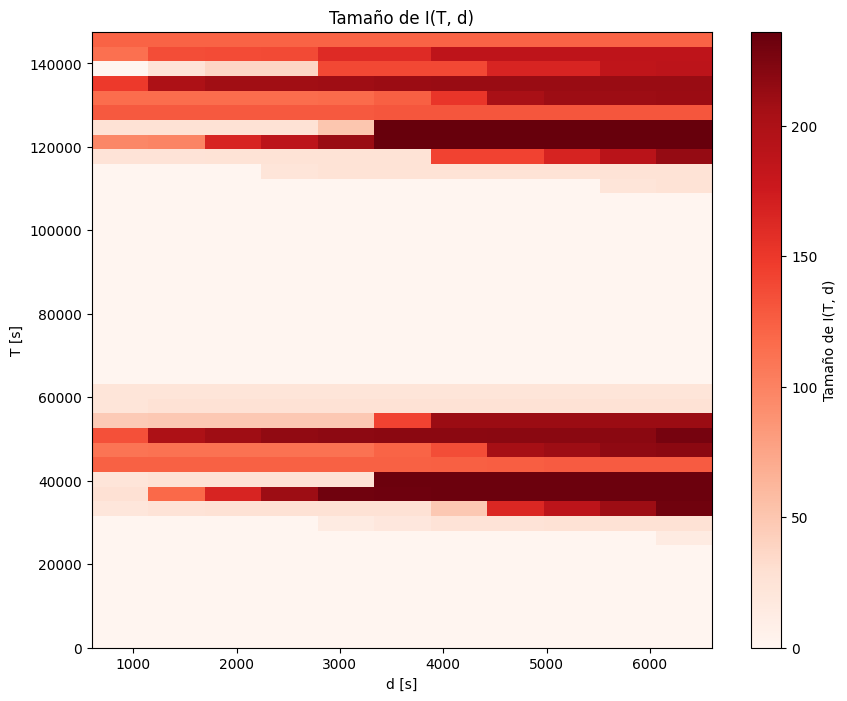
\includegraphics[scale=0.4]{images/influencia.png}
                \caption{Influencia de estudiante 1695}
                \label{fig:influencia}
            \end{figure}
            Los períodos con mayor actividad social, o influencia, están representados por los colores más oscuros en el gráfico, lo que sugiere que existen momentos específicos durante el día donde la influencia del estudiante es mayor, los que pueden relacionarse con recreos, actividades grupales, entre otros.

            También es posible notar los períodos de baja actividad social del estudiante, representados por los colores más claros en el gráfico, que pueden estar relacionados con momentos en los que el estudiante no se encuentra en la escula, por ejemplo. El análisis de los períodos con mayor y menor actividad social permiten identificar los patrones de influencia, que además proporcionan información sobre la dinámica de esta red.

            Finalmente, al observar estos patrones de influencia en función del tiempo y la duración de estas interacciones es posible notar los momentos claves que podrían ser útiles para un estudio más detallado o intervención.
        \end{enumerate}
\end{itemize}
\end{document}